\section{Flow and Diffusion Models}
\label{sec:odes_sdes}
In the previous section, we formalized generative modeling as sampling from a data distribution $\pdata$. Further, we saw that sampling could be achieved via the transformation of samples from a simple distribution $\pinit$, such as the Gaussian $\mathcal{N}(0,I_d)$, to samples from the target distribution $\pdata$. In this section, we describe how the desired transformation can be obtained as the simulation of a suitably constructed differential equation. For example, flow matching and diffusion models involve simulating \themebf{ordinary differential equations} (ODEs) and \themebf{stochastic differential equations} (SDEs), respectively. The goal of this section is therefore to define and construct these generative models as they will be used throughout the remainder of the notes. Specifically, we first define ODEs and SDEs, and discuss their simulation. Second, we describe how to parameterize an ODE/SDE using a deep neural network. This leads to the definition of a flow and diffusion model and the fundamental algorithms to sample from such models. In later sections, we then explore how to train these models.

% \paragraph{Note.} We remark that there are other ways to transform $\pinit$ into $\pdata$ other than ODEs/SDEs. We focus on ODEs/SDEs because they represent the current state-of-the-art but just keep in mind that many other ways have been proposed over the course of the history of machine learning offering unique advantages and disadvantages.

\subsection{Flow Models}

We start by defining \themebf{ordinary differential equations (ODEs)}. A solution to an ODE is defined by a \themebf{trajectory}, i.e. a function of the form
\begin{align*}
X: [0,1] \to \R^d, \quad t \mapsto X_t,
\end{align*}
that maps from time $t$ to some location in space $\mathbb{R}^d$. Every ODE is defined by a \themebf{vector field} $u$, i.e. a function of the form
\begin{align*}
u:\mathbb{R}^d\times [0,1]\to \R^d,\quad (x,t)\mapsto u_t(x),
\end{align*}
i.e. for every time $t$ and location $x$ we get a vector $u_t(x)\in\R^d$ specifying a velocity in space (see  \cref{fig:flow}). An ODE imposes a condition on a trajectory: we want a trajectory $X$ that ``follows along the lines'' of the vector field $u_t$, starting at the point $x_0$. We may formalize such a trajectory as being the solution to the equation:
\begin{subequations}
    \begin{align} 
      \frac{\dd}{\dd t}X_{t} &= u_t(X_t) &&\blacktriangleright\,\,\text{ODE}\label{e:ode_ode}\\
      X_0&= x_0            &&\blacktriangleright\,\,\text{initial conditions}\label{e:ODE_boundary} 
    \end{align}
\end{subequations}
\Cref{e:ode_ode} requires that the derivative of $X_t$ is specified by the direction given by $u_t$. \Cref{e:ODE_boundary} requires that we start at $x_0$ at time $t=0$. We may now ask: if we start at $X_0 = x_0$ at $t=0$, where are we at time $t$ (what is $X_t$)? This question is answered by a function called the \themebf{flow}, which is a solution to the ODE
\begin{subequations}\label{e:flow}
    \begin{align}
    \psi:\R^d\times [0,1]\mapsto& \R^d,\quad (x_0,t)\mapsto \psi_t(x_0)\\
      \frac{\dd}{\dd t}\psi_{t}(x_0) &= u_t(\psi_{t}(x_0)) &&\blacktriangleright\,\, \text{flow ODE}\label{e:flow_flow}\\
      \psi_{0}(x_0)             &= x_0                &&\blacktriangleright\,\,\text{flow initial conditions}\label{e:flow_boundary} 
    \end{align}
\end{subequations}
For a given initial condition $X_0=x_0$, a trajectory of the ODE is recovered via $X_t = \psi_t(X_0)$. Therefore, vector fields, ODEs, and flows are, intuitively, three descriptions of the same object: \textbf{vector fields define ODEs whose solutions are flows}. As with every equation, we should ask ourselves about an ODE: Does a solution exist and if so, is it unique? A fundamental result in mathematics is "yes!" to both, as long we impose weak assumptions on $u_t$:

\begin{theorem}[Flow existence and uniqueness]
\label{thm:ode_existence_and_uniqueness}
If $u:\R^d\times[0,1]\to\R^d$ is continuously differentiable with a bounded derivative, then the ODE in \eqref{e:flow} has a unique solution given by a flow $\psi_t$. In this case, $\psi_t$ is a \themebf{diffeomorphism} for all $t$, i.e. $\psi_t$ is continuously differentiable with a continuously differentiable inverse $\psi_t^{-1}$.
\end{theorem}
Note that the assumptions required for the existence and uniqueness of a flow are almost always fulfilled in machine learning, as we use neural networks to parameterize $u_t(x)$ and they always have bounded derivatives. Therefore, \cref{thm:ode_existence_and_uniqueness} should not be a concern for you but rather good news: \textbf{flows exist and are unique solutions to ODEs in our cases of interest.} A proof can be found in \citep{perko2013differential,coddington1956theory}.

\begin{figure}
    \centering
    \begin{tabular}{ccc}
         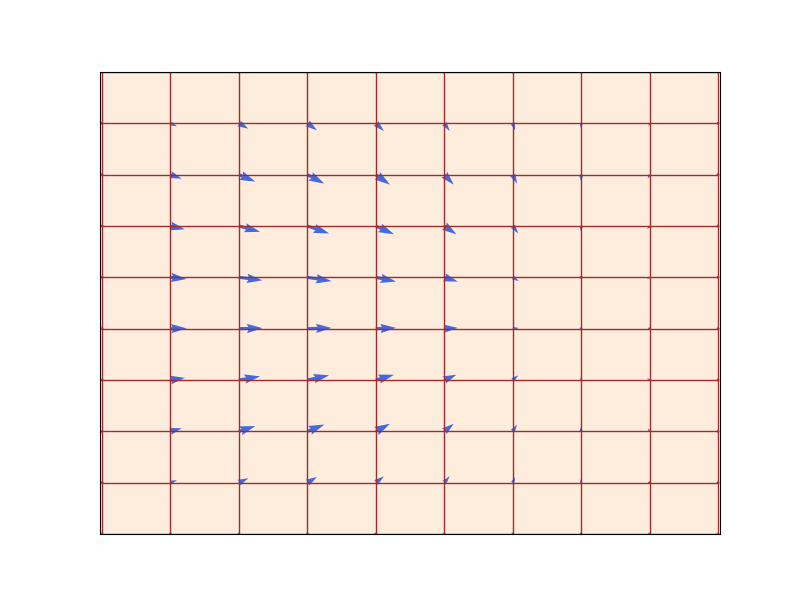
\includegraphics[width=0.3\textwidth]{fm_guide_assets/flow_1.png} &
         % \includegraphics[width=0.22\textwidth]{assets/flow_velocity/flow_v_5.png} &
         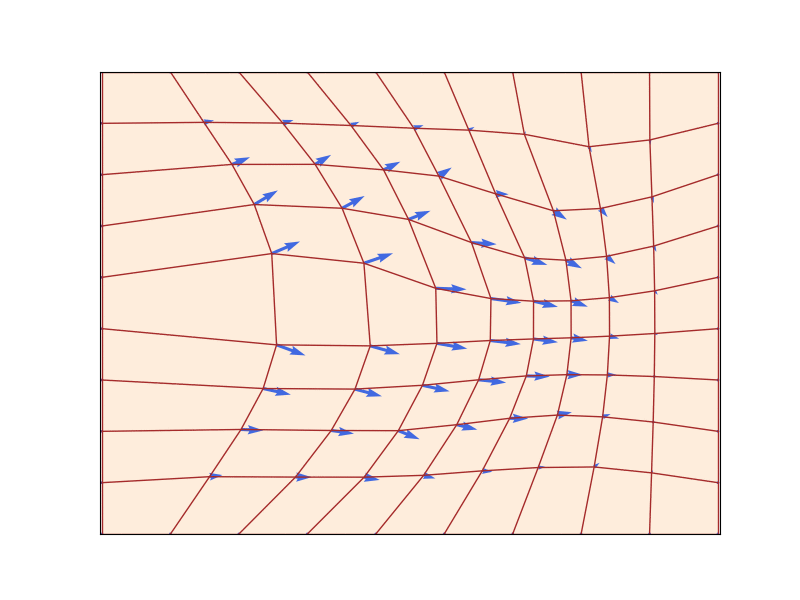
\includegraphics[width=0.3\textwidth]{fm_guide_assets/flow_10.png} &
         % \includegraphics[width=0.22\textwidth]{assets/flow_velocity/flow_v_14.png} &
         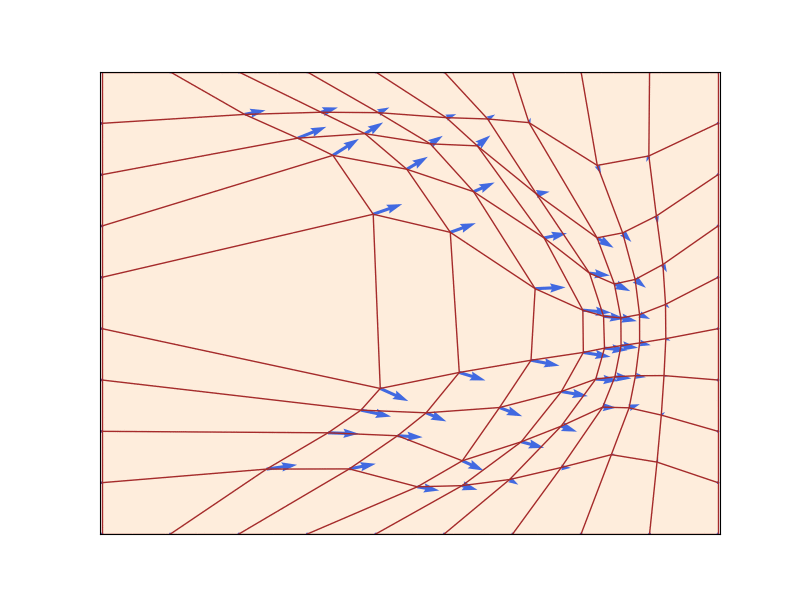
\includegraphics[width=0.3\textwidth]{fm_guide_assets/flow_16.png} 
    \end{tabular}
    \caption{A flow $\psi_t:\Real^d\too \Real^d$ (red square grid) is defined by a velocity field $u_t :\Real^d\too\Real^d$ (visualized with blue arrows) that prescribes its instantaneous movements at all locations (here, $d=2$). We show three different times $t$. As one can see, a flow is a diffeomorphism that "warps" space. Figure from \citep{lipman2024flow}.}
    \label{fig:flow}
\end{figure}

\begin{examplebox}[Linear Vector Fields]
Let us consider a simple example of a vector field $u_t(x)$ that is a simple linear function in $x$, i.e. $u_t(x)=-\theta x$ for $\theta>0$. Then the function
\begin{align}
    \label{e:flow_linear_vf}
    \psi_t(x_0) =  \exp\left(-\theta t\right)x_0
\end{align}
defines a flow $\psi$ solving the ODE in \cref{e:flow}. You can check this yourself by checking that $\psi_0(x_0)=x_0$ and computing
\begin{align*}
    \frac{\dd}{\dd t}\psi_t(x_0) \overset{\eqref{e:flow_linear_vf}}{=}\frac{\dd}{\dd t}\left(\exp\left(-\theta t\right)x_0\right)
    \overset{(i)}{=}-\theta\exp\left(-\theta t\right)x_0\overset{\eqref{e:flow_linear_vf}}{=}-\theta\psi_t(x_0)=u_t(\psi_t(x_0)),
\end{align*}
where in (i) we used the chain rule. In \cref{fig:bm_ou_process}, we visualize a flow of this form converging to $0$ exponentially.
\end{examplebox}

\paragraph{Simulating an ODE.}
In general, it is not possible to compute the flow $\psi_t$ explicitly if $u_t$ is not as simple as a linear function. In these cases, one uses \themebf{numerical methods} to simulate ODEs. Fortunately, this is a classical and well researched topic in numerical analysis, and a myriad of powerful methods exist \citep{iserles2009first}. One of the simplest and most intuitive methods is the \themebf{Euler method}. In the Euler method, we initialize with $X_0=x_0$ and update via
\begin{equation}
\label{e:euler_method}
X_{t+h} = X_t + h u_t(X_t)\quad (t=0,h,2h,3h,\dots,1-h)
\end{equation}
where $h=n^{-1}>0$ is a step size hyperparameter with $n \in \Nat$. For this class, the Euler method will be good enough. To give you a taste of a more complex method, let us consider \themebf{Heun's method} defined via the update rule
\begin{alignat*}{3}
    X_{t+h}'&=X_t+hu_t(X_t)\quad &&\blacktriangleright\,\, \text{initial guess of new state}\\
    X_{t+h} &= X_{t} + \frac{h}{2}(u_t(X_t)+u_{t+h}(X_{t+h}'))\quad &&\blacktriangleright\,\,\text{update with average $u$ at current and guessed state}
\end{alignat*}
Intuitively, the Heun's method is as follows: it takes a first guess $X_{t+h}'$ of what the next step could be but corrects the direction initially taken via an updated guess.

\paragraph{Flow models.} We can now construct a generative model via an ODE. Remember that our goal was to convert a simple distribution $\pinit$ into a complex distribution $\pdata$. The simulation of an ODE is thus a natural choice for this transformation. A \themebf{flow model} is described by the ODE
\begin{align*}
    X_0 &\sim \pinit  &&\blacktriangleright\,\,\text{random initialization} \\
    \frac{\dd}{\dd t}X_t &= u_t^\theta(X_t) &&\blacktriangleright\,\,\text{ODE}
\end{align*}
where the vector field $u_t^\theta$ is a neural network $u_t^\theta$ with parameters $\theta$. For now, we will speak of $u_t^\theta$ as being a generic neural network; i.e. a continuous function $u_t^\theta:\mathbb{R}^d\times [0,1]\to\mathbb{R}^d$ with parameters $\theta$. Later, we will discuss particular choices of neural network architectures. Our goal is to make the endpoint  $X_1$ of the trajectory have distribution $\pdata$, i.e.
\begin{align*}
    X_1 \sim \pdata \quad \Leftrightarrow \quad \psi_1^\theta(X_0)\sim \pdata
\end{align*}
where $\psi_t^\theta$ describes the flow induced by $u_t^\theta$. Note however: although it is called \themeit{flow model}, \textbf{the neural network parameterizes the vector field, not the flow}. In order to compute the flow, we need to simulate the ODE. In \cref{alg:sampling_flow_model}, we summarize the procedure how to sample from a flow model.

\begin{algorithm}[h]
\caption{Sampling from a Flow Model with Euler method}
\label{alg:sampling_flow_model}
\begin{algorithmic}[1]
\REQUIRE Neural network vector field $u_t^\theta$, number of steps $n$
\STATE Set $t=0$
\STATE Set step size $h=\frac{1}{n}$
\STATE Draw a sample $X_0\sim \pinit$
\FOR{$i=1,\dots,n-1$}
    \STATE $X_{t+h} = X_{t} + h u_t^\theta(X_t)$
    \STATE Update $t\leftarrow t+h$
\ENDFOR
\RETURN $X_1$
\end{algorithmic}
\end{algorithm}

% \paragraph{Flow generative model.}\ph{Potentially leave out this section. We explain the SDE generative model} We can now construct a generative model via flows. A first attempt might be to construct a neural network that approximates a flow $\psi_t$ directly. However, this turns out to be pretty hard as $\psi_t$ has to be a diffeomorphism, which is a hard constraint to enforce on neural networks (if you are interested, you should look up \emph{normalizing flows} \citep{kobyzev2020normalizing}). Instead, it is much simpler to define a neural network that parameterizes a vector field
% \begin{align*}
%     \textbf{Neural Network: }u^\theta:\R^d\times [0,1]\to \R^d, (t,x)\mapsto u_t^\theta(x)\text{  with parameters }\theta
% \end{align*}
% We can equivalently write $\psi_t^\theta$ for the corresponding flow. However, you should always keep in mind that we can only compute $\psi_t^\theta$ by simulating an ODE with the neural network $u_t^\theta$. Therefore, to obtain samples from our \themebf{flow generative model}, the procedure is as follows:
% \begin{align*}
% \textbf{Initialization:}\quad X_0\sim&\pinit \quad  &&(\text{"Initialize with simple distribution, e.g. a Gaussian"})\\
%     \textbf{Simulation:}\quad \frac{\dd}{\dd t}X_t=&u_t^\theta(X_t)\quad &&(\text{"Simulate ODE from 0 to 1, e.g. using Euler method"})\\
%     \textbf{Goal:}\quad X_1 \sim & \pdata \quad &&(\text{"Goal is to make }X_1\text{ have distribution }\pdata\text{"})
% \end{align*}
% Note that the only source of randomness in a flow model is the initial point $X_0\sim \pinit$ - the remaining evolution is deterministic. Further, note that the simulating of the ODE will always incur an error (i.e. we will never be able to compute $\psi_1^\theta$ precisely). However, this is an error that we can usually control by choosing a good ODE solver and simply reducing the step size $h$ in \cref{e:euler_method}.



\subsection{Diffusion Models}
Stochastic differential equations (SDEs) extend the deterministic trajectories from ODEs with \themebf{stochastic} trajectories. A stochastic trajectory is commonly called a \themebf{stochastic process} $(X_t)_{0\leq t\leq 1}$ and is given by
\begin{align*}
    X_t \text{ is a random variable for every } 0\leq t\leq 1\\
    X: [0,1] \to \R^d, \quad t \mapsto X_t\text{ is a random trajectory for every draw of }X
\end{align*}
In particular, when we simulate the same stochastic process twice, we might get different outcomes because the dynamics are designed to be random.

\paragraph{Brownian Motion.} SDEs are constructed via a \themebf{Brownian motion} - a fundamental stochastic process that came out of the study physical diffusion processes. You can think of a Brownian motion as a continuous random walk.
\begin{wrapfigure}{r}{0.4\textwidth}
  %\begin{center}
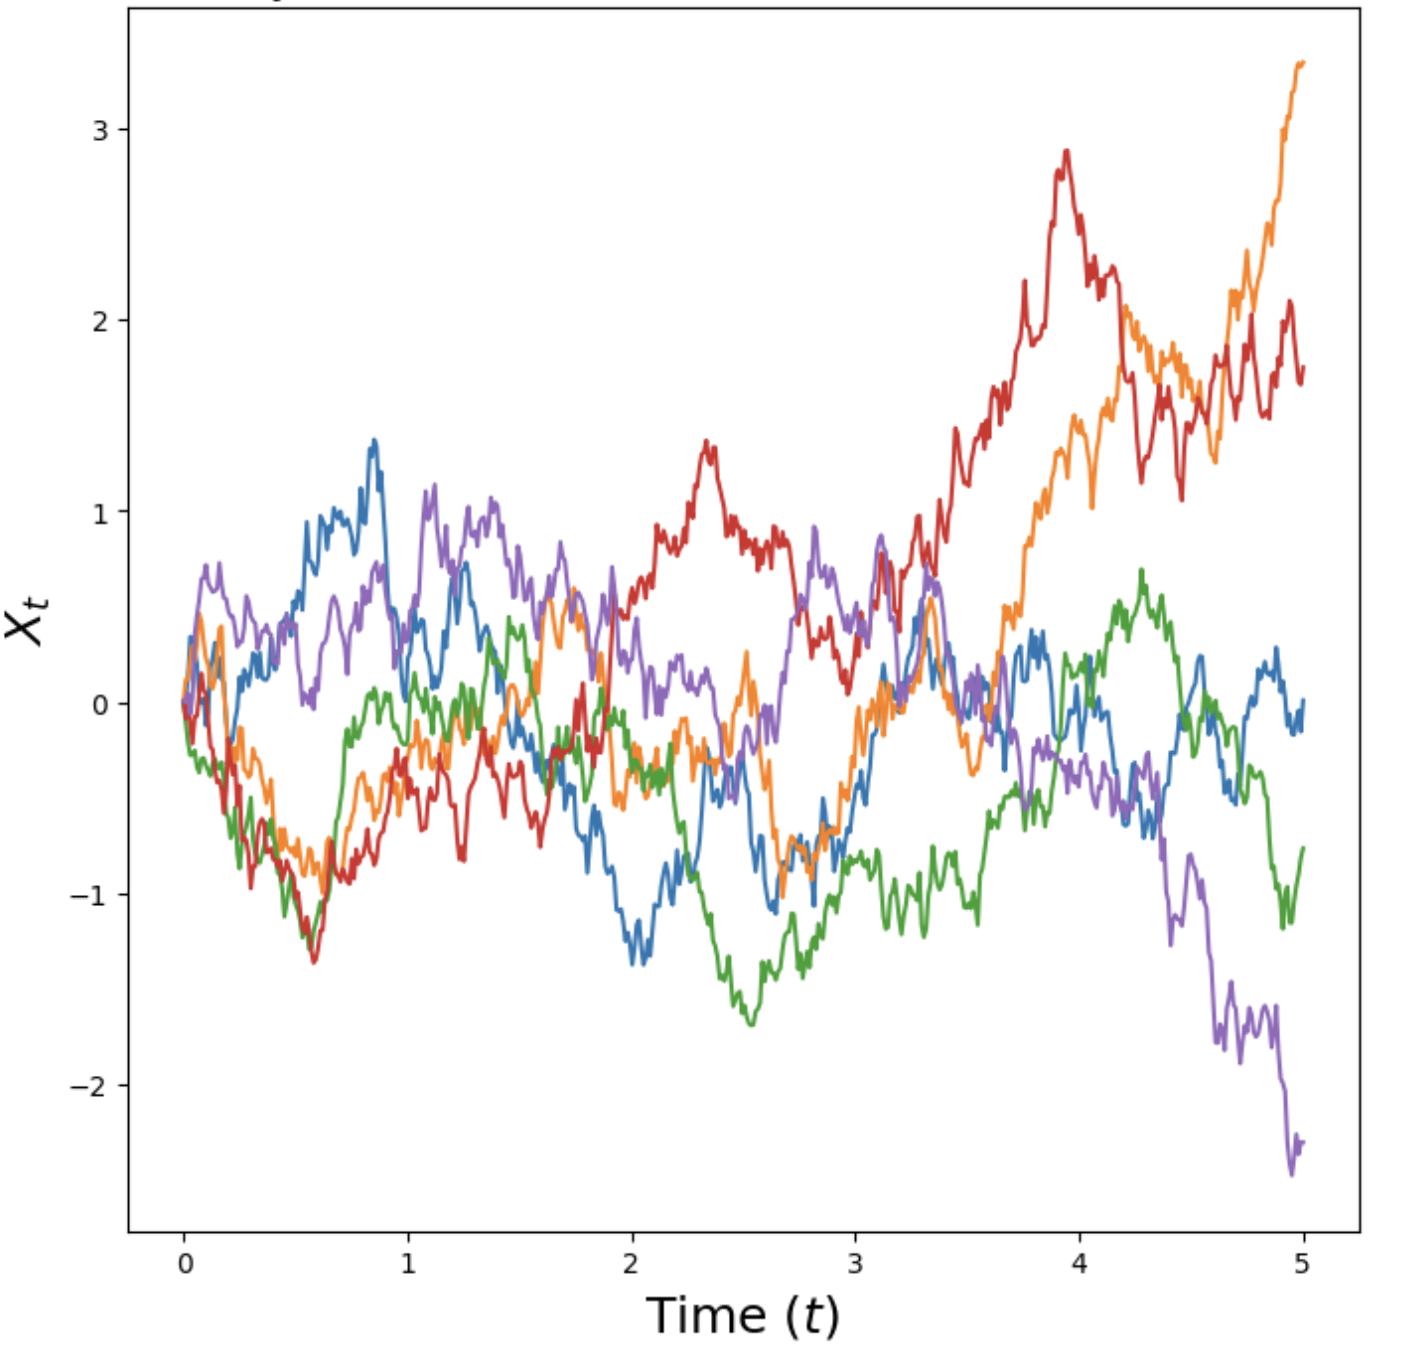
\includegraphics[width=0.4\textwidth]{figures/brownian_motion_sample_paths.png}
  %\end{center}
  \vspace{-20pt}
  \caption{Sample trajectories of a Brownian motion $W_t$ in dimension $d=1$ simulated using \cref{eq:brownian_motion_simulation}.}
  \label{fig:brownian_motion_trajectories}
  \vspace{-10pt}
\end{wrapfigure}
Let us define it: A \themebf{Brownian motion} $W = (W_t)_{0\leq t\leq 1}$ is a stochastic process such that $W_0=0$, the trajectories $t\mapsto W_t$ are continuous, and the following two conditions hold:
\begin{enumerate}
    \item \textbf{Normal increments: }$W_{t}-W_{s}\sim \mathcal{N}(0,(t-s)I_d)$ for all $0\leq s<t$, i.e. increments have a Gaussian distribution with variance increasing linearly in time ($I_d$ is the identity matrix).
    \item \textbf{Independent increments: }For any $0\leq t_0<t_1<\dots <t_n=1$, the increments $W_{t_1}-W_{t_0},\dots,W_{t_n}-W_{t_{n-1}}$ are independent random variables.
\end{enumerate}

Brownian motion is also called a \themebf{Wiener process}, which is why we denote it with a "$W$".\footnote{Nobert Wiener was a famous mathematician who taught at MIT. You can still see his portraits hanging at the MIT math department.} We can easily simulate a Brownian motion approximately with step size $h>0$ by setting $W_0=0$ and updating
\begin{align}
    \label{eq:brownian_motion_simulation}
    W_{t+h} =& W_{t} + \sqrt{h}\epsilon_t,\quad \epsilon_t\sim\mathcal{N}(0,I_d)\quad (t=0,h,2h,\dots,1-h)
\end{align}
In \cref{fig:brownian_motion_trajectories}, we plot a few example trajectories of a Brownian motion.  Brownian motion is as central to the study of stochastic processes as the Gaussian distribution is to the study of probability distributions. From finance to statistical physics to epidemiology, the study of Brownian motion has far reaching applications beyond  machine learning. In finance, for example, Brownian motion is used to model the price of complex financial instruments. Also just as a mathematical construction, Brownian motion is fascinating: For example, while the paths of a Brownian motion are continuous (so that you could draw it without ever lifting a pen), they are infinitely long (so that you would never stop drawing).
%Furhter (2) Any continuous-time Markov process with zero mean and independent, stationary increments is automatically a Brownian motion.

\begin{figure}
    \centering
    \begin{tabular}{ccc}
         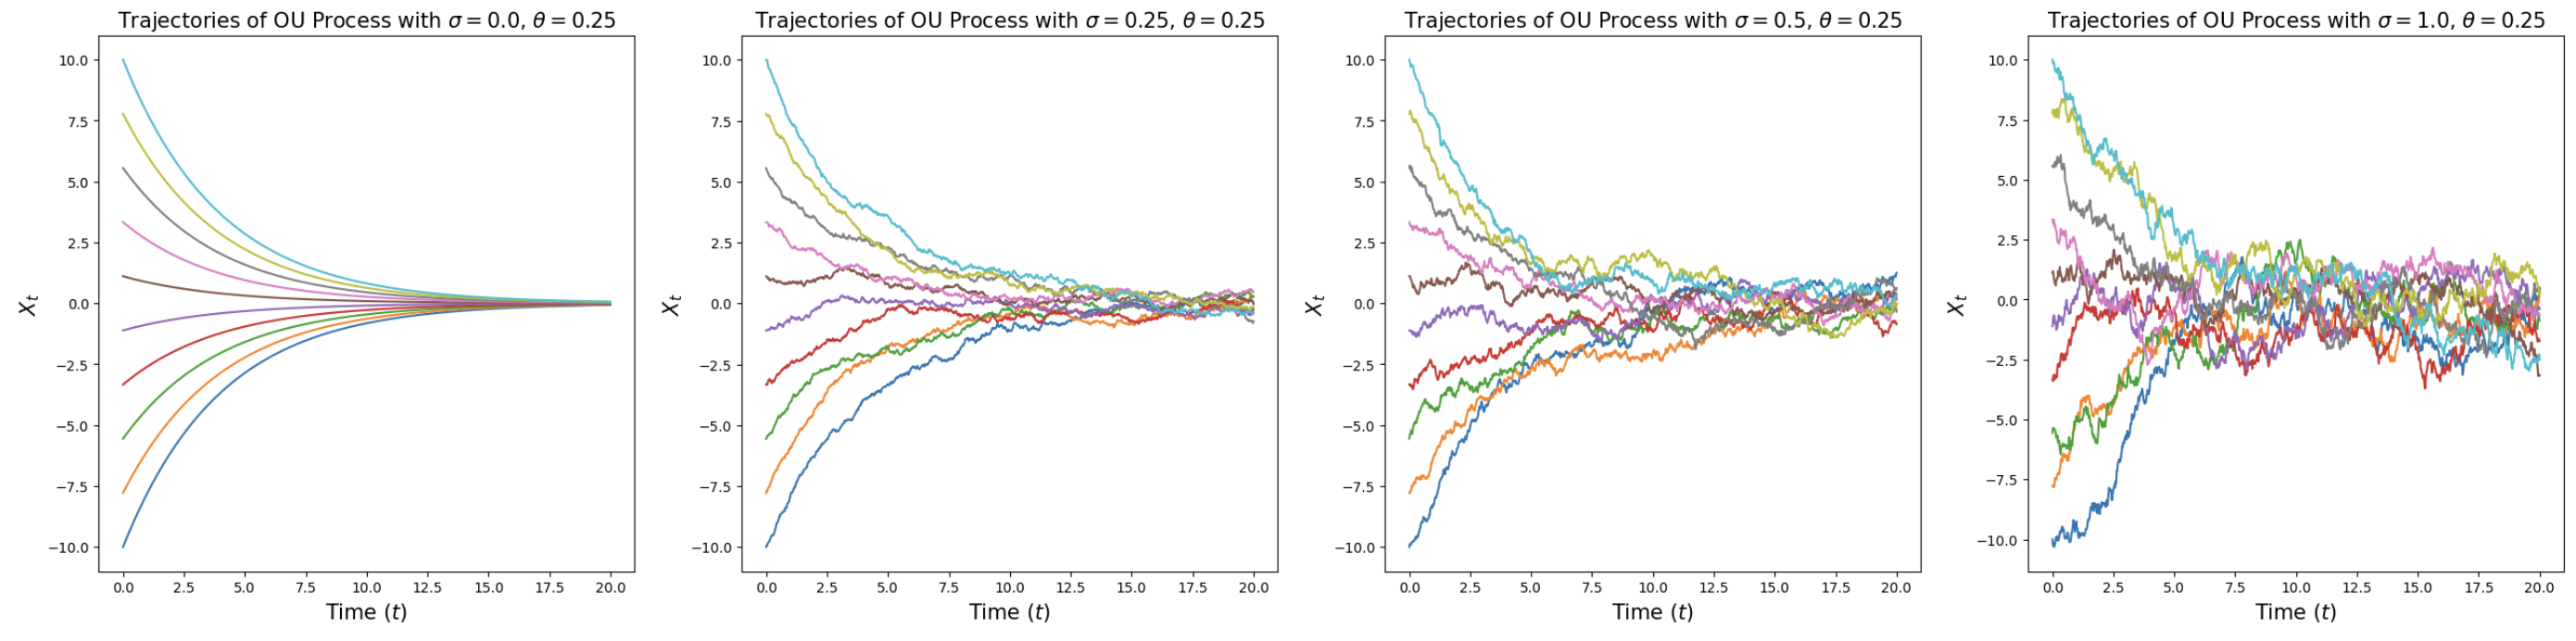
\includegraphics[width=\textwidth]{figures/ou_process.png} &
         % \includegraphics[width=0.22\textwidth]{assets/flow_velocity/flow_v_5.png} &
         % 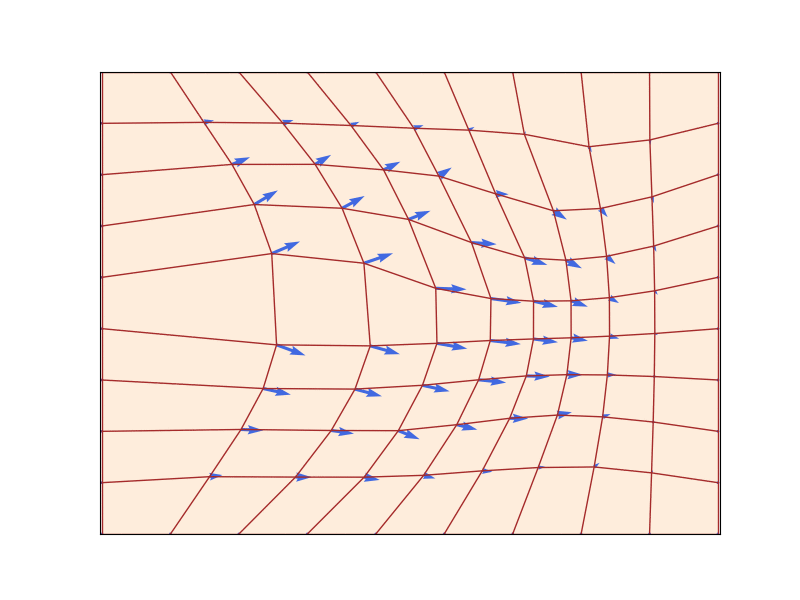
\includegraphics[width=0.3\textwidth]{fm_guide_assets/flow_10.png} &
         % % \includegraphics[width=0.22\textwidth]{assets/flow_velocity/flow_v_14.png} &
         % 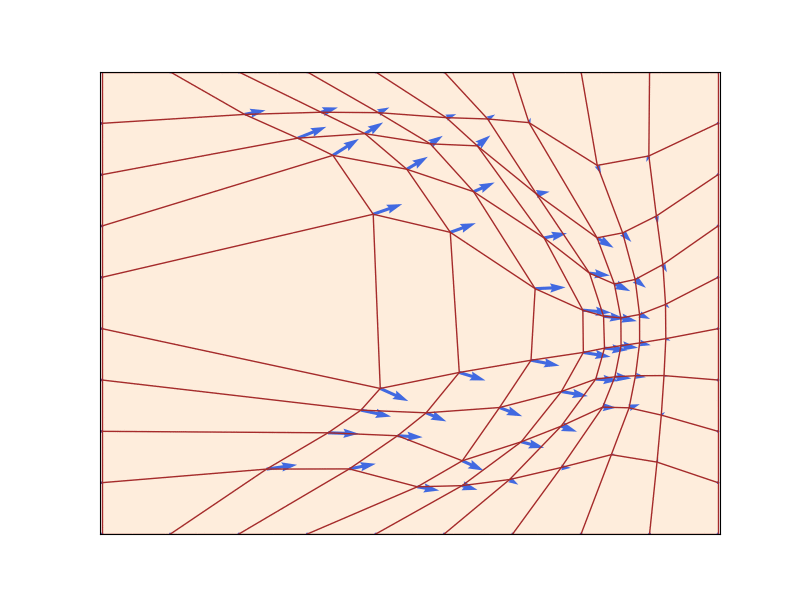
\includegraphics[width=0.3\textwidth]{fm_guide_assets/flow_16.png} 
    \end{tabular}
    \caption{\label{fig:bm_ou_process} Illustration of Ornstein-Uhlenbeck processes (\cref{eq:ohrstein_uhlenbeck_process}) in dimension $d=1$ for $\theta=0.25$ and various choices of $\sigma$ (increasing from left to right). For $\sigma=0$, we recover a flow (smooth, deterministic trajectories) that converges to the origin as $t \to \infty$. For $\sigma>0$ we have random paths which converge towards the Gaussian $\mathcal{N}(0,\frac{\sigma^2}{2\theta})$ as $t\to\infty$.}
\end{figure} 

\paragraph{From ODEs to SDEs.} The idea of an SDE is to extend the deterministic dynamics of an ODE by adding stochastic dynamics driven by a Brownian motion. Because everything is stochastic, we may no longer take the derivative as in \cref{e:ode_ode}. Hence, we need to find an \textbf{equivalent formulation of ODEs that does not use derivatives}. For this, let us therefore rewrite trajectories $(X_t)_{0\leq t\leq 1}$ of an ODE as follows:
\begin{alignat*}{3}
    \frac{\dd}{\dd t} X_t &=  u_t(X_t) \quad &&\blacktriangleright\,\,\text{expression via derivatives}\\
    \overset{(i)}{\Leftrightarrow} \quad  \frac{1}{h}\left(X_{t+h}-X_{t}\right)&=u_t(X_t) + R_t(h)&&\\
\Leftrightarrow \quad X_{t+h} &= X_{t}+hu_t(X_t) + hR_t(h)\quad &&\blacktriangleright\,\,\text{expression via infinitesimal updates}
\end{alignat*}
where  $R_t(h)$ describes a negligible function for small $h$, i.e. such that $\lim\limits_{h\to 0}R_t(h)=0$, and in $(i)$ we simply use the definition of derivatives. The derivation above simply restates what we already know: A trajectory $(X_t)_{0 \le t \le 1}$ of an ODE takes, at every timestep, a small step in the direction $u_t(X_t)$. We may now amend the last equation to make it stochastic: A trajectory $(X_t)_{0 \le t \le 1}$ of an SDE takes, at every timestep, a small step in the direction $u_t(X_t)$ \themeit{plus} some contribution from a Brownian motion:
\begin{align}
    \label{e:infinitesimal_updates_sdes}
    X_{t+h} = X_{t}+\underbrace{hu_t(X_t)}_{\text{deterministic}} + \sigma_t\underbrace{(W_{t+h}-W_{t})}_{\text{stochastic}}+\underbrace{hR_t(h)}_{\text{error term}}
\end{align}
where $\sigma_t\geq 0$ describes the \themebf{diffusion coefficient} and $R_t(h)$ describes a stochastic error term such that the standard deviation $\mathbb{E}[\|R_t(h)\|^2]^{1/2}\to 0$ goes to zero for $h\to 0$. The above describes a \themebf{stochastic differential equation (SDE)}. It is common to denote it in the following symbolic notation:
\begin{subequations}\label{e:sde_generic}
    \begin{align} 
      \dd X_t &= u_t(X_t)\dd t + \sigma_t\dd W_t &&\blacktriangleright\,\,\text{SDE}\\
      X_0 &= x_0               &&\blacktriangleright\,\,\text{initial condition}
    \end{align}
\end{subequations}
However, always keep in mind that the "$\dd X_t$"-notation above is a purely informal notation of \cref{e:infinitesimal_updates_sdes}. Unfortunately, SDEs do not have a flow map $\phi_t$ anymore. This is because the value $X_t$ is not fully determined by $X_0\sim \pinit$ anymore as the evolution itself is stochastic. Still, in the same way as for ODEs, we have:
\begin{theorem}[SDE Solution Existence and Uniqueness]
\label{thm:sde_existence_and_uniqueness}
If $u:\R^d\times[0,1]\to\R^d$ is continuously differentiable with a bounded derivative and $\sigma_t$ is continuous, then the SDE in \eqref{e:sde_generic} has a solution given by the unique stochastic process $(X_t)_{0\leq t\leq 1}$ satisfying \cref{e:infinitesimal_updates_sdes}.
\end{theorem}
If this was a stochastic calculus class, we would spend several lectures proving this theorem and constructing SDEs with full mathematical rigor, i.e. constructing a Brownian motion from first principles and constructing the process $X_{t}$ via \themebf{stochastic integration}. As we focus on machine learning in this class, we refer to \citep{mao2007stochastic} for a more technical treatment. Finally, note that every ODE is also an SDE - simply with a vanishing diffusion coefficient $\sigma_t=0$. Therefore, for the remainder of this class, \textbf{when we speak about SDEs, we consider ODEs as a special case}.
% \begin{remarkbox}[A Note on Formality]
% If this was a stochastic calculus class, we would spend more time constructing SDEs with full mathematical rigor, i.e. constructing a Brownian motion from first principles and constructing the process $X_{t}$ via \emph{stochastic integrals}. \ee{Revise: Those of you familiar with stochastic calculus will note that our discussion of SDEs has thus far been quite informal. For example, we have technically not actually shown that a Brownian motion even exists. If this were a class on stochastic calculus, we might proceed more formally, by e.g., constructing a Brownian motion and then arriving at SDEs via the notion of a \themeit{stochastic integral}. Nevertheless, we feel that this extra machinery is overly cumbersome for the need at hand, and have therefore opted to take a more direct approach.}
% \end{remarkbox}

\begin{examplebox}[Ornstein-Uhlenbeck Process]
Let us consider a constant diffusion coefficient $\sigma_t=\sigma\geq 0$ and a constant linear drift $u_t(x)=-\theta x$ for $\theta>0$, yielding the SDE
\begin{align}
\label{eq:ohrstein_uhlenbeck_process}
\dd X_t = -\theta X_t\dd t + \sigma dW_t.
\end{align} 
A solution $(X_t)_{0 \le t \le 1}$ to the above SDE is known as an \themebf{Ornstein-Uhlenbeck (OU) process}. We visualize it in \cref{fig:bm_ou_process}. The vector field $-\theta x$ pushes the process back to its center $0$ (as I always go the inverse direction of where I am), while the diffusion coefficient $\sigma$ always adds more noise. This process converges towards a Gaussian distribution $\mathcal{N}(0,\sigma^2)$ if we simulate it for $t\to \infty$. Note that for $\sigma=0$, we have a flow with linear vector field that we have studied in \cref{e:flow_linear_vf}.
\end{examplebox}


\paragraph{Simulating an SDE.} If you struggle with the abstract definition of an SDE so far, then don't worry about it. A more intuitive way of thinking about SDEs is given by answering the question: How might we simulate an SDE? The simplest such scheme is known as the \themebf{Euler-Maruyama method}, and is essentially to SDEs what the Euler method is to ODEs. Using the Euler-Maruyama method, we initialize $X_0=x_0$ and update iteratively via
\begin{align}
\label{e:euler_method_sdes}
    X_{t+h} = X_{t}+hu_t(X_t) + \sqrt{h}\sigma_t\epsilon_t,\quad \quad \epsilon_t \sim \mathcal{N}(0,I_d)
\end{align}
where $h=n^{-1}>0$ is a step size hyperparameter for $n \in \Nat$. In other words, to simulate using the Euler-Maruyama method, we take a small step in the direction of $u_t(X_t)$ as well as add a little bit of Gaussian noise scaled by $\sqrt{h}\sigma_t$. When simulating SDEs in this class (such as in the accompanying labs), we will usually stick to the Euler-Maruyama method.

\begin{algorithm}[h]
\caption{Sampling from a Diffusion Model (Euler-Maruyama  method)}
\label{alg:sampling_diffusion_model}
\begin{algorithmic}[1]
\REQUIRE Neural network $u_t^\theta$, number of steps $n$, diffusion coefficient $\sigma_t$
\STATE Set $t=0$
\STATE Set step size $h=\frac{1}{n}$
\STATE Draw a sample $X_0\sim \pinit$
\FOR{$i=1,\dots,n-1$}
    \STATE Draw a sample $\epsilon\sim \mathcal{N}(0,I_d)$
    \STATE $X_{t+h} = X_{t} + h u_t^\theta(X_t)+\sigma_t\sqrt{h}\epsilon$
    \STATE Update $t\leftarrow t+h$
\ENDFOR
\RETURN $X_1$
\end{algorithmic}
\end{algorithm}

\paragraph{Diffusion Models.} We can now construct a generative model via an SDE in the same way as we did for ODEs. Remember that our goal was to convert a simple distribution $\pinit$ into a complex distribution $\pdata$. Like for ODEs, the simulation of an SDE randomly initialized with $X_0\sim \pinit$ is a natural choice for this transformation. To parameterize this SDE, we can simply parameterize its central ingredient - the vector field $u_t$ - a neural network $u_t^\theta$. A \themebf{diffusion model} is thus given by
\begin{align*}
    \dd X_t &= u_t^\theta(X_t)\dd t + \sigma_t \dd W_t &&\blacktriangleright\,\,\text{SDE}\\
    X_0 &\sim \pinit  &&\blacktriangleright\,\,\text{random initialization}
    \end{align*}
In \cref{alg:sampling_diffusion_model}, we describe the procedure by which to sample from a diffusion model with the Euler-Maruyama method. We summarize the results of this section as follows.
\begin{summarybox}[SDE generative model] Throughout this document, a \themebf{diffusion model} consists of a neural network $u_t^\theta$ with parameters $\theta$ that parameterize a vector field and a fixed  diffusion coefficient $\sigma_t$:
\begin{align*}
    \textbf{\sffamily Neural network: }&u^\theta:\R^d\times [0,1]\to \R^d,\,\, (x,t)\mapsto u_t^\theta(x)\text{  with parameters }\theta\\
    \textbf{\sffamily Fixed: }&\sigma_t:[0,1]\to [0,\infty),\,\, t\mapsto \sigma_t
\end{align*}
To obtain samples from our SDE model (i.e. generate objects), the procedure is as follows:
\begin{align*}
\textbf{\sffamily Initialization:}\quad X_0&\sim\pinit \quad  &&\blacktriangleright\,\,\text{Initialize with simple distribution, e.g. a Gaussian}\\
    \textbf{\sffamily Simulation:}\quad \dd X_t &= u_t^\theta(X_t)\dd t + \sigma_t\dd W_t\quad &&\blacktriangleright\,\,\text{Simulate SDE from 0 to 1}\\
    \textbf{\sffamily Goal:}\quad X_1 &\sim  \pdata \quad &&\blacktriangleright\,\,\text{Goal is to make $X_1$ have distribution $\pdata$}
\end{align*}
A diffusion model with $\sigma_t=0$ is a \themebf{flow model}.
\label{summary:diffusion_model}
\end{summarybox}